% THIS DOCUMENT IS FOLLOWS THE VOLERE TEMPLATE BY Suzanne Robertson and James Robertson
% ONLY THE SECTION HEADINGS ARE PROVIDED
%
% Initial draft from https://github.com/Dieblich/volere
%
% Risks are removed because they are covered by the Hazard Analysis
\documentclass[12pt]{article}

\usepackage{booktabs}
\usepackage{tabularx}
\usepackage{hyperref}
\usepackage{float}
\usepackage{graphicx}
\usepackage{longtable}
\hypersetup{
    bookmarks=true,         % show bookmarks bar?
      colorlinks=true,      % false: boxed links; true: colored links
    linkcolor=red,          % color of internal links (change box color with linkbordercolor)
    citecolor=green,        % color of links to bibliography
    filecolor=magenta,      % color of file links
    urlcolor=cyan           % color of external links
}

\newcommand{\lips}{\textit{Insert your content here.}}

%% Comments

\usepackage{color}

\newif\ifcomments\commentstrue %displays comments
%\newif\ifcomments\commentsfalse %so that comments do not display

\ifcomments
\newcommand{\authornote}[3]{\textcolor{#1}{[#3 ---#2]}}
\newcommand{\todo}[1]{\textcolor{red}{[TODO: #1]}}
\else
\newcommand{\authornote}[3]{}
\newcommand{\todo}[1]{}
\fi

\newcommand{\wss}[1]{\authornote{blue}{SS}{#1}} 
\newcommand{\plt}[1]{\authornote{magenta}{TPLT}{#1}} %For explanation of the template
\newcommand{\an}[1]{\authornote{cyan}{Author}{#1}}

%% Common Parts

\newcommand{\progname}{Software Engineering} % PUT YOUR PROGRAM NAME HERE
\newcommand{\authname}{Team \#11, OKKM Insights
\\ Mathew Petronilho
\\ Oleg Glotov
\\ Kyle McMaster
\\ Kartik Chaudhari} % AUTHOR NAMES                  

\usepackage{hyperref}
    \hypersetup{colorlinks=true, linkcolor=blue, citecolor=blue, filecolor=blue,
                urlcolor=blue, unicode=false}
    \urlstyle{same}
                                


\begin{document}

\title{Software Requirements Specification for \progname: subtitle describing software} 
\author{\authname}
\date{\today}
	
\maketitle

~\newpage

\pagenumbering{roman}

\tableofcontents

~\newpage

\section*{Revision History}

\begin{tabularx}{\textwidth}{p{3cm}p{2cm}X}
\toprule {\textbf{Date}} & {\textbf{Version}} & {\textbf{Notes}}\\
\midrule
10/1/2024 & Mathew Petronilho & Added Purpose Of Project\\
Date 2 & 1.1 & Notes\\
\bottomrule
\end{tabularx}

~\\

~\newpage
\section{Purpose of the Project}
There is currently a lack of high-quality, labeled satellite imagery datasets tailored for specific use cases. Many industries require specialized data for tasks like disaster 
response, environmental monitoring, urban planning, or defense, but building these datasets manually is time-consuming, costly, inefficient and may require expert data analysis. 
This hinders the development and deployment of accurate computer vision models for critical use cases across these various industries.

The purpose of this project is to create an online platform that accelerates this process and brings simplicity to satellite imagery data analysis.
\subsection{Goals of the Project}
\subsubsection{High Data Accuracy}
The system should have high classification accuracy for objects reported in the images. The core problem this system must solve is extracting useful information from the provided images.
 One key metric to determine the utility of the information found, is the classification accuracy of objects identified in the images. If the system is 
 not able to determine what is contained in an image, it will not be useful to stakeholders.
\subsubsection{Ease of use}
The system should be very easy for stakeholders to use. There should be very low friction for users to classify images and objects found
within images, with minimal training. It should also be simple for users to upload images to be analyzed. To maximize the information gained from users who are contributing to classification efforts, the system must ensure it is simple for users to 
get started with, and continue using the system. This is necessary to build a large enough user base, which will make it more likely to get insights in an acceptable 
amount of time.
\subsubsection{Minimizing Cost to Analyze Images}
The system should minimize the cost for users request insights from images. This could be implemented through intelligent algorithms for task delegation. Users of the system who upload images are interested in getting an appropriate return for their investment. If the cost to analyze is too high, the platform will not
retain a sufficiently large user base of purchasers.
\subsubsection{Results Returned Within Appropriate Timeframe}
The system should ensure the time it takes to obtain information from images is within a specified limit, as determined by users who upload images. Purchasers will have some time limit they require the system to process images within. To ensure timing needs are met, the system should provide realistic timelines and stick to them.
\subsubsection{High System Reliability and Accessibility}
The system should be useable remotely for purchasers and labellers, and have minimal downtime.The system should allow purchasers to upload images without being physically located where the system is hosted to ensure flexibility of use. The same should also be true for labellers, as they 
should be able to perform their tasks remotely. In both cases, the system should have low down time as to not introduce additional friction into the completion of tasks.
\section{Stakeholders}
\subsection{Client}
\lips
\subsection{Customer}
\lips
\subsection{Other Stakeholders}
\lips
\subsection{Hands-On Users of the Project}
\lips
\subsection{Personas}
\lips
\subsection{Priorities Assigned to Users}
\lips
\subsection{User Participation}
\lips
\subsection{Maintenance Users and Service Technicians}
\lips

\section{Mandated Constraints}
\begin{itemize}
  \item The solution must be fully compatible with the latest stable releases of Google Chrome, Firefox, Microsoft Edge, and Safari browsers.\\ \textbf{Rationale:} Users will interact with the web application through various modern web browsers, so ensuring cross-browser compatibility is essential for providing a consistent user experience. \\ \textbf{Fit Criteria:} The web application must display consistently, maintain full functionality, and support core features across all specified browsers without major visual or functional discrepancies. Testing should be conducted on each browser to validate compatibility.
\end{itemize}
\subsection{Implementation Environment of the Current System}
There is no current environment in which our application must be implemented.
\subsection{Partner or Collaborative Applications}
There are no constraints regarding external applications that must be used alongside our product.
\subsection{Off-the-Shelf Software}
There is no required off-the-shelf software that must be used for our application.
\subsection{Anticipated Workplace Environment}
There is no particular location where users are required to work and use the product. As a web application, it can be accessed from most computers with an internet connection. We do not anticipate that the users' environment will physically constrain their ability to use the app in any way.
\subsection{Schedule Constraints}
\begin{itemize}
  \item The proof of concept for this project must be ready to demonstrate by \textbf{November 11, 2024}. Not meeting this deadline will result in uncertainty about overcoming major risks associated with the project.
  \item The first project demonstration must be ready by \textbf{February 3, 2025}. Missing this deadline will reduce the time available to make refinements based on feedback and findings.
  \item The final demonstration must be ready by \textbf{March 24, 2025}. Missing this milestone would prevent the project from being presented and result in a significant loss of marks.
\end{itemize}
To see other documentation deadlines related to this project, refer to our \href{https://github.com/OKKM-insights/OKKM.insights/blob/main/docs/DevelopmentPlan/DevelopmentPlan.pdf}{Development Plan}. 
\subsection{Budget Constraints}
\begin{itemize}
  \item The project budget must not exceed \$750. All funds will be sourced from the team itself.
\end{itemize}

\section{Naming Conventions and Terminology}
\subsection{Glossary of All Terms, Including Acronyms, Used by Stakeholders
involved in the Project}
\begin{table}[H]
    \centering
    \begin{tabular}{|p{0.3\linewidth} | p{0.7\linewidth}| }
    \hline
    \textbf{Term} & \textbf{Definition}\\
    \hline
    Labellers & Users of our application that will be labeling photos shown to them for a monetary reward\\
    \hline
    \end{tabular}
    \caption{Naming Conventions and Terminology}
\end{table}

\section{Relevant Facts And Assumptions}
\subsection{Relevant Facts}
\lips
\subsection{Business Rules}
\lips
\subsection{Assumptions}
\lips

\section{The Scope of the Work}
\subsection{The Current Situation}
\lips
\subsection{The Context of the Work}
\lips
\subsection{Work Partitioning}
\lips
\subsection{Specifying a Business Use Case (BUC)}
\lips

\section{Business Data Model and Data Dictionary}
\subsection{Business Data Model}
\lips
\subsection{Data Dictionary}
\lips

\section{The Scope of the Product}
\subsection{Product Boundary}
The use case diagram depicted below identifies the boundaries between the users and the product.
\begin{figure}[H]
    \centering
    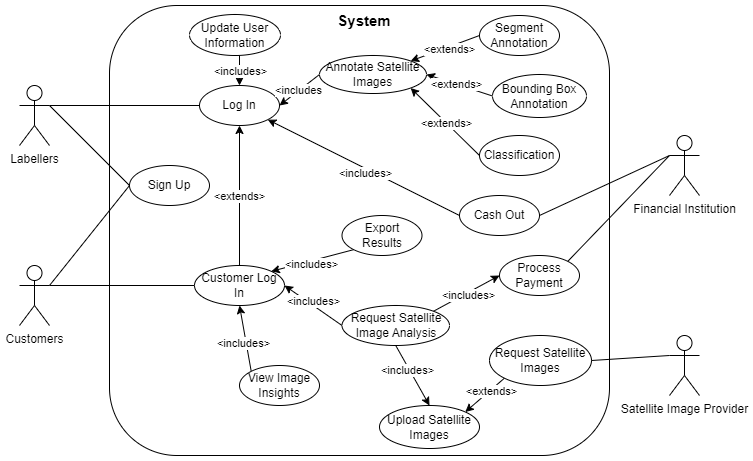
\includegraphics[scale=0.63]{useCaseDiagram.png}
    \caption{Use Case diagram}
    \label{fig:usecase}
\end{figure}
\subsection{Product Use Case Table}
\begin{longtable}
 {p{0.1\textwidth} | p{0.35\textwidth} | p{0.2\textwidth} | p{0.35\textwidth}}
  \toprule
  \textbf{PUC No} & \textbf{PUC Name} & \textbf{Actor/s} & \textbf{Input \& Output}\\
  \midrule
  1 & Sign Up & Labellers, Customers & Personal information \& credentials (in), New account (out)\\
  \midrule
  2 & Log In & Labellers & Credentials (in)\\
  \midrule
  3 & Customer Log In & Customers & Credentials (in)\\
  \midrule
  4 & Update User Information & Labellers, Customers & Information to change (in),  Updated information (out)\\
   \midrule
  5 & Annotate Images & Labellers & Image \& annotation (in), Labelled image (out)\\
  \midrule
  6 & Segment Annotation & Labellers & Segmented image \& user selections (in), Image with labelled segments (out)\\
  \midrule
  7 & Bounding Box Annotation & Labellers & Image \& box annotations (in), Image with labelled boxes (out)\\
  \midrule
  8 & Classification & Labellers & Image \& choices (in), Image labelled with the selected choice (out)\\
  \midrule
   9 & Cash Out & Labellers, Financial Institution & Financial information (in), Payment to user (out)\\
  \midrule
  10 & View Image Insights & Customers & Request to view insights (in), Image insights (out)\\
  \midrule
  11 & Export Results & Customers & Request to export results (in), Results in downloadable format (out)\\
  \midrule
  12 & Request Image Analysis & Customers & Labels, images \& examples (in) \\
  \midrule
  13 & Upload Images & Customers & Images (in)\\
  \midrule
  14 & Request Images & Customers, Satellite Image Provider & Description of images wanted (in), Images (out)\\
  \midrule
  15 & Process Payment & Customers, Financial Institution & Financial information (in), Payment to app (out)\\
  \bottomrule
  \caption{Product Use Cases} \label{TblPUC}\\
\end{longtable}
\subsection{Individual Product Use Cases (PUC's)}
\subsubsection{PUC 1 - Sign Up}
\textbf{Primary Actors:} Labellers, Customers\\ 
\textbf{Precondition:} None\\
\textbf{Trigger:} User selects create an account\\
\textbf{Success Scenario:}
\begin{enumerate}
    \item User provides the required information and agrees with the privacy policy of the application
    \item System verifies all required information has been provided and is of valid syntax
    \item System securely registers the given information
    \item User is directed to the login page
\end{enumerate}
\textbf{Post-condition:} User has successfully created an account and the application has securely stored their information

\subsubsection{PUC 2 - Log In}
\textbf{Primary Actors:} Labellers\\ 
\textbf{Precondition:} Labeller has signed up for an account\\
\textbf{Trigger:} Labeller selects log in\\
\textbf{Success Scenario:}
\begin{enumerate}
    \item Labeller enters credentials
    \item System verifies all required information has been provided and matches the stored records
    \item Labeller is redirected to the home page as a logged-in user
\end{enumerate}
\textbf{Post-condition:} The labeller has access to their account. All account related information, such as labeling progress, is accurately represented

\subsubsection{PUC 3 - Customer Log In}
\textbf{Primary Actors:} Customers\\ 
\textbf{Precondition:} Customer has signed up for an account\\
\textbf{Trigger:} Customer selects log in\\
\textbf{Success Scenario:}
\begin{enumerate}
    \item Customer enters credentials
    \item System verifies all required information has been provided and matches the stored records
    \item Customer is redirected to the home page as a logged-in customer, which gives them access to more features than a labeller
\end{enumerate}
\textbf{Post-condition:} The customer has access to their account and all their current image analysis projects

\subsubsection{PUC 4 - Update User Information}
\textbf{Primary Actors:} Labellers, Customers\\ 
\textbf{Precondition:} User has logged in\\
\textbf{Trigger:} User selects update information\\
\textbf{Success Scenario:}
\begin{enumerate}
    \item User enters updated information
    \item System verifies the new information has valid syntax
    \item System updates the information
    \item User is given a confirmation that their information has been updated
\end{enumerate}
\textbf{Post-condition:} The information that the system stores about the user has been updated

\subsubsection{PUC 5 - Annotate Images}
\textbf{Primary Actors:} Labellers\\ 
\textbf{Precondition:} Labeller has logged in\\
\textbf{Trigger:} Labeller selects a listed project\\
\textbf{Success Scenario:}
\begin{enumerate}
    \item An image related to the selected project and a description of what to annotate is shown to the labeller
    \item The labeller annotates the image to the best of their ability
    \item The annotated image is submitted by the labeller
    \item The labeller is rewarded and the image is stored by the system
    \item If the labeller skips the image rather than submits it, then the annotated image will not be stored by the system and the labeller will not receive a reward
    \item The next image of the selected project is shown to the labeller and the process repeats
\end{enumerate}
\textbf{Post-condition:} All submitted annotated images are stored by the system. The labeller's reward balance is updated to reflect their submissions

\subsubsection{PUC 6 - Segment Annotation}
\textbf{Primary Actors:} Labellers\\ 
\textbf{Precondition:} Labeller has logged in\\
\textbf{Trigger:} Labeller selects a listed project\\
\textbf{Success Scenario:}
\begin{enumerate}
    \item The same as Annotate Images, but the labeller is given a image segmented into different parts and must label each segment to the best of their ability 
\end{enumerate}
\textbf{Post-condition:} All submitted annotated images are stored by the system. The labeller's reward balance is updated to reflect their submissions

\subsubsection{PUC 7 - Bounding Box Annotation}
\textbf{Primary Actors:} Labellers\\ 
\textbf{Precondition:} Labeller has logged in\\
\textbf{Trigger:} Labeller selects a listed project\\
\textbf{Success Scenario:}
\begin{enumerate}
    \item The same as Annotate Images, but the labeller must annotate areas of the image by drawing boxes and providing a label for each box
\end{enumerate}
\textbf{Post-condition:} All submitted annotated images are stored by the system. The labeller's reward balance is updated to reflect their submissions

\subsubsection{PUC 8 - Classification}
\textbf{Primary Actors:} Labellers\\ 
\textbf{Precondition:} Labeller has logged in\\
\textbf{Trigger:} Labeller selects a listed project\\
\textbf{Success Scenario:}
\begin{enumerate}
    \item The same as Annotate Images, but the labeller must classify what category an image belongs to given several options
\end{enumerate}
\textbf{Post-condition:} All submitted annotated images are stored by the system. The labeller's reward balance is updated to reflect their submissions

\subsubsection{PUC 9 - Cash Out}
\textbf{Primary Actors:} Labellers\\
\textbf{Secondary Actor:} Financial Institution\\
\textbf{Precondition:} Labeller has logged in and their reward balance is at least \$1\\
\textbf{Trigger:} Labeller selects cash out\\
\textbf{Success Scenario:}
\begin{enumerate}
    \item The system retrieves the labeller's payment information
    \item The labeller confirms it is correct, or updates their information accordingly
    \item The system sends a payment to the labeller through their financial institution
    \item The labeller's reward balance is set back to \$0
\end{enumerate}
\textbf{Post-condition:} The financial account that the labeller provided has gained money equal to the labeller's reward balance

\subsubsection{PUC 10 - View Image Insights}
\textbf{Primary Actors:} Customers\\
\textbf{Precondition:} Customer has logged in and has at least one image analysis project\\
\textbf{Trigger:} Customer selects insights for a project\\
\textbf{Success Scenario:}
\begin{enumerate}
    \item The system provides the customer with a progress update, key statistics, and an overview of current labels for specific images
    \item The customer selects a specific image to view insights 
    \item The system gets the information it has stored related to the image and provides insights such as confidence level of annotations
\end{enumerate}
\textbf{Post-condition:} The customer has knowledge about how their project is progressing and if the labeling of the images has been complete

\subsubsection{PUC 11 - Export Results}
\textbf{Primary Actors:} Customers\\
\textbf{Precondition:} Customer has logged in, has at least one image analysis project, and all labeled images in that project have an acceptable accuracy\\
\textbf{Trigger:} Customer selects export data\\
\textbf{Success Scenario:}
\begin{enumerate}
    \item The system retrieves all the labeled images associated with the project
    \item The system asks the customer where they would like the images to be saved
    \item The customer specifies the save location
    \item The images are downloaded to the specified location
\end{enumerate}
\textbf{Post-condition:} The customer has complete access to the labeled dataset of images

\subsubsection{PUC 12 - Request Image Analysis}
\textbf{Primary Actors:} Customers\\
\textbf{Precondition:} Customer has logged in\\
\textbf{Trigger:} Customer creates a new project request\\
\textbf{Success Scenario:}
\begin{enumerate}
    \item The system prompts the customer with a form to fill out regarding information about the project such as what is to be labelled
    \item The customer fills out the form and submits it
    \item The system confirms the forms information is valid. It prompts the customer to upload the image dataset to be analyzed
    \item The customer uploads their own images or requests the system to get images for them
    \item The system asks the customer to provide sample labelled images that can be shared with labellers
    \item The customer uploads sample labelled images
    \item Based on the size and difficulty of the project, the system provides the total cost of the project to the customer
    \item The customer provides their payment details
    \item The system processes the payment
    \item The system makes the project available to labellers so they can annotate the images
\end{enumerate}
\textbf{Post-condition:} The image analysis project has been created and labellers can start annotating the images

\subsubsection{PUC 13 - Upload Images}
\textbf{Primary Actors:} Customers\\
\textbf{Precondition:} Customer has logged in and has created a new project request\\
\textbf{Trigger:} Customer submits the information form for a new project\\
\textbf{Success Scenario:}
\begin{enumerate}
    \item The system prompts the customer to upload the images they would like to be analyzed
    \item The customer selects the images they want analyzed and uploads them
    \item The system stores the images with a reference to the project
\end{enumerate}
\textbf{Post-condition:} The system has all the images that will be analyzed for the project

\subsubsection{PUC 14 - Request Images}
\textbf{Primary Actors:} Customers\\
\textbf{Secondary Actors:} Satellite Image Provider\\
\textbf{Precondition:} Customer has logged in and has created a new project request\\
\textbf{Trigger:} Customer submits the information form for a new project\\
\textbf{Success Scenario:}
\begin{enumerate}
    \item The system prompts the customer about the type of images they want. This could be satellite images from a specific time frame in a specific area
    \item The customer specifies the type of images they want for analysis
    \item The system contacts a satellite image provider, and pays a fee to them in exchange for the images. The fee is charged to the customer
    \item The system stores the images with a reference to the project
\end{enumerate}
\textbf{Post-condition:} The system has all the images that will be analyzed for the project

\subsubsection{PUC 15 - Process Payment}
\textbf{Primary Actors:} Customers\\
\textbf{Secondary Actor:} Financial Institution\\
\textbf{Precondition:} Customer has logged in and has created a new project request\\
\textbf{Trigger:} Customer has filled out all the details of the project and uploaded all the photos\\
\textbf{Success Scenario:}
\begin{enumerate}
    \item The system retrieves the customer's payment information
    \item The customer confirms it is correct, or updates their information accordingly
    \item The system sends a payment request to the customer's financial institution
    \item The financial institution validates the payment information and sends the payment
    \item The payment is deposited in the financial account associated with the system
\end{enumerate}
\textbf{Post-condition:} The fees for facilitating the project have been paid

\section{Functional Requirements}
\subsection{Functional Requirements}
\lips

\section{Look and Feel Requirements}
\subsection{Appearance Requirements}
\subsubsection*{Requirement LF1:}
\begin{itemize}
  \item \textbf{Description:} The application shall adapt to various screen sizes, ensuring legibility and an uncluttered layout.
  \item \textbf{Rationale:} Users will have computers with varying screen sizes, so a consistent experience across all these sizes is ideal.
  \item \textbf{Fit Criterion:} Visual elements must not exceed the boundaries of a screen with a size between the range 1024×768 pixels to 1920×1080 pixels.
\end{itemize}
\subsubsection*{Requirement LF2:}
\begin{itemize}
  \item \textbf{Description:} Interactive elements such as buttons shall provide visual feedback to the user.
  \item \textbf{Rationale:} This will allow users a better understanding of when their actions have been processed by the application.
  \item \textbf{Fit Criterion:} Every interactive element changes colour or displays additional visual cues, such as animations or shadows, to indicate interaction.
\end{itemize}
\subsection{Style Requirements}
\subsubsection*{Requirement LF3:}
\begin{itemize}
  \item \textbf{Description:} The application should maintain a unified visual design across all components.
  \item \textbf{Rationale:} A consistent appearance enhances the application's cohesiveness and conveys a professional aesthetic.
  \item \textbf{Fit Criterion:} Font type, sizing, and colour, along with background tones are all consistent throughout the application.
\end{itemize}

\section{Usability and Humanity Requirements}
\subsection{Ease of Use Requirements}
\lips
\subsection{Personalization and Internationalization Requirements}
\lips
\subsection{Learning Requirements}
\lips
\subsection{Understandability and Politeness Requirements}
\lips
\subsection{Accessibility Requirements}
\lips

\section{Performance Requirements}
\subsection{Speed and Latency Requirements}
\lips
\subsection{Safety-Critical Requirements}
\lips
\subsection{Precision or Accuracy Requirements}
\lips
\subsection{Robustness or Fault-Tolerance Requirements}
\lips
\subsection{Capacity Requirements}
\lips
\subsection{Scalability or Extensibility Requirements}
\lips
\subsection{Longevity Requirements}
\lips

\section{Operational and Environmental Requirements}
\subsection{Expected Physical Environment}
\lips
\subsection{Wider Environment Requirements}
\lips
\subsection{Requirements for Interfacing with Adjacent Systems}
\lips
\subsection{Productization Requirements}
\lips
\subsection{Release Requirements}
\lips

\section{Maintainability and Support Requirements}
\subsection{Maintenance Requirements}
\subsubsection*{NFR-MR1}
\begin{itemize}
  \item \textbf{Description:} All maintainance required for the system shall be possible to complete by a competent software developer after reading all of the documentation provided in the source repository.
  \item \textbf{Rationale:} The system should be well documented, and therefore maintainable after reading said documents.
  \item \textbf{Fit Criterion:} A competent software developer, as determined by the original developers or their agents, can solve problems related to the core of the system, as determined by the 
  features outlined in this document.
\end{itemize}
\subsection{Supportability Requirements}
N/A
\subsection{Adaptability Requirements}
N/A

\section{Security Requirements}
\subsection{Access Requirements}
\subsubsection*{Requirement SR1:}
\begin{itemize}
  \item \textbf{Description:} The application shall only allow users with labeling access, including labellers, customers, and admins, to view active projects and label images.
  \item \textbf{Rationale:} We do not want random users with no stake in the process to effect the results.
  \item \textbf{Fit Criterion:} Users who have not logged in to the application have no way of viewing projects or labeling images. Users logged in as labellers, customers, or admins have access to these features.
\end{itemize}
\subsubsection*{Requirement SR2:}
\begin{itemize}
  \item \textbf{Description:} The application shall only allow users with customer access and above to create new image analysis projects.
  \item \textbf{Rationale:} Unidentified users creating projects would be impossible to facilitate. Also, labellers have no need to access project creation. 
  \item \textbf{Fit Criterion:} Users who have not logged in to the application have no way of creating an image analysis project. Users logged in as customers or admins have access to these features.
\end{itemize}
\subsubsection*{Requirement SR3:}
\begin{itemize}
  \item \textbf{Description:} The application shall validate the email format the user provides when creating an account.
  \item \textbf{Rationale:} We do not want users using invalid emails to sign up.
  \item \textbf{Fit Criterion:} Let E represent the set of all email addresses, and let V represent the set of all valid email addresses. A valid email address conforms to the general pattern:\\\\
  V = $(\forall\; email \in E\;  |\; email \; matches \; the \; pattern \; $[a-zA-Z0-9+\_.-]+@[a-zA-Z0-9.-]+[a-zA-Z])\\
\end{itemize}
\subsubsection*{Requirement SR4:}
\begin{itemize}
  \item \textbf{Description:} The application shall validate the password format the user provides when creating an account.
  \item \textbf{Rationale:} We do not want users using weak passwords to sign up.
  \item \textbf{Fit Criterion:} Let P represent the set of all passwords, and let V represent the set of all valid passwords. A valid password has a at least one lowercase, uppercase, number and special character and is a minimum of 8 characters in length:\\\\
  V = $(\forall\; password \in P\;  |\; password \; matches \; the \; pattern \; $(?=.*[a-z])(?=.*[A-Z])(?=.*[0-9])(?=.*[\#\$\%\&\*\@])[a-zA-Z0-9\#\$\%\&\*\@]\{8,\})\\
\end{itemize}
\subsection{Integrity Requirements}
\subsubsection*{Requirement SR5:}
\begin{itemize}
  \item \textbf{Description:} The application shall prevent incorrect data from being introduced.
  \item \textbf{Rationale:} The database of information should always reflect correct and up to date information.
  \item \textbf{Fit Criterion:} The system must validate user inputs for data accuracy and format before they are saved. Any invalid data must trigger error messages, preventing it from being entered into the database. Users must be required to correct errors before proceeding.
\end{itemize}
\subsection{Privacy Requirements}
\subsubsection*{Requirement SR6:}
\begin{itemize}
  \item \textbf{Description:} User data will be securely encrypted to protect user’s privacy.
  \item \textbf{Rationale:} This will help to avoid user's being compromised if a data leak occurs.
  \item \textbf{Fit Criterion:} An encryption algorithm is used on sensitive user data such as passwords.
\end{itemize}
\subsubsection*{Requirement SR7:}
\begin{itemize}
  \item \textbf{Description:} The application shall ensure that all payment transactions are processed securely using encryption and comply with relevant security standards, such as PCI-DSS, which helps to protect payment account data (PCI Security Standards Council, 2024).
  \item \textbf{Rationale:} Protecting users' financial information is critical to maintaining trust. Failing to secure payments can lead to data breaches, financial loss, and legal liabilities.
  \item \textbf{Fit Criterion:} All payment transactions must use industry-standard encryption to protect sensitive data. Payment information, such as credit card details, must not be stored locally on the application and must be processed via a secure, PCI-DSS-compliant third-party payment gateway.
\end{itemize}

\subsection{Audit Requirements}
These requirements are not applicable as we are not an organization that is currently subject to audits.
\subsection{Immunity Requirements}
\subsubsection*{Requirement SR8:}
\begin{itemize}
  \item \textbf{Description:} The application shall use parameterized queries or prepared statements for all database interactions.
  \item \textbf{Rationale:} We want to prevent SQL injection attacks which can lead to unauthorized data access or manipulation.
  \item \textbf{Fit Criterion:} All database queries must be implemented using parameterized queries or prepared statements. Dynamic SQL strings that concatenate user input must not be used in the codebase.
\end{itemize}

\section{Cultural Requirements}
\subsection{Cultural Requirements}
\subsubsection*{NFR-CUR1}
\begin{itemize}
  \item \textbf{Description:} The system shall present users with the option to select the most popular language in each country it is deployed in.
  \item \textbf{Rationale:} It is important that the users of the program can understand what is said in each step.
  \item \textbf{Fit Criterion:} A drop down will allow users to select from the list of languages. At a minimum, the most popular language by number of speakers will be available for each country.
\end{itemize}

\section{Compliance Requirements}
\subsection{Legal Requirements}
\lips
\subsection{Standards Compliance Requirements}
\lips

\section{Open Issues}
\textbf{Task Assignment Algorithm: }To ensure labelers are engaged as they complete tasks and to obtain the highest quality of information possible, the system must implement an intelligent task allocation system. This system has not yet been determined.
\\\textbf{Label Consensus Algorithm: }Similarly, the algorithm for combining multiple user labels into one accurate label has not yet been determined. 
\\\textbf{Labeling Services Offered: }The system has determined several potential labeling services to be offered by the system, but has not confirmed with certainty what will be included. This will be determined after more research has been completed on the task assignment algorithm.

\section{Off-the-Shelf Solutions}
\subsection{Ready-Made Products}
\textbf{Amazon Mechanical Turk: } A web-based crowdsourcing platform. Instead of building a novel front end, the system could obtain labels through this platform instead.
\subsection{Reusable Components}
\textbf{Label Studio: } A React library which contains components for building a web-based data annotation platform.
\subsection{Products That Can Be Copied}
\textbf{Tolka AI: } A general purpose image label crowdsourcing site. Supports image segmentation, bounding box drawing, and more computer vision labeling tasks.



\section{New Problems}
\subsection{Effects on the Current Environment}
The introduction of the OKKM Insights platform is expected to have several impacts on the existing technological and operational environment.
\subsubsection{Data Privacy and Security Concerns}
\begin{enumerate}
    \item Impact: Handling sensitive satellite imagery and user-generated data raises significant privacy and security issues. Ensuring compliance with data protection regulations is paramount.
    \item Potential Problem: Breaches or mishandling of data could lead to legal repercussions, loss of trust, and reputational damage.
\end{enumerate}
\subsubsection{Environmental Footprint}
\begin{enumerate}
    \item Impact: Increased computational requirements for AI processing and data storage may lead to higher energy consumption.
    \item Potential Problem: This could conflict with sustainability goals and lead to higher operational costs.
\end{enumerate}
\subsection{Effects on the Installed Systems}
Introducing the OKKM Insights platform will interact with and potentially disrupt existing systems within the organization and for stakeholders.
\subsubsection{Integration Challenges}
\begin{enumerate}
    \item Impact: The platform will need to integrate with existing data sources, cloud services, and possibly applicable third-party APIs.
    \item Potential Problem: Incompatibilities or integration failures could result in data inconsistencies, system downtimes, or increased maintenance efforts.
\end{enumerate}
\subsubsection{Legacy Systems Compatibility}
\begin{enumerate}
    \item Impact: Older systems may not support the latest technologies required by the new platform.
    \item Potential Problem: Upgrading or adjusting to legacy systems can be costly and time-consuming, potentially delaying the platform's deployment.
\end{enumerate}
\subsection{Potential User Problems}
Users are at the heart of the OKKM Insights platform, and several issues may arise that affect their experience and satisfaction.
\subsubsection{Usability Issues}
\begin{enumerate}
    \item Impact: If the platform is not intuitive or user-friendly, users may struggle to navigate and utilize its features effectively.
    \item Potential Problem: Poor user experience can lead to reduced engagement, lower data labeling contributions, and higher dropout rates.
\end{enumerate}
\subsubsection{Training and Onboarding}
\begin{enumerate}
    \item Impact: Users may require training to understand how to label data accurately and use the platform's tools.
    \item Potential Problem: Inadequate training resources can result in inconsistent labeling, decreasing the quality of the datasets and the reliability of the AI models.
\end{enumerate}
\subsubsection{Compensation and Incentives}
\begin{enumerate}
    \item Impact: Users expect fair compensation for their contributions.
    \item Potential Problem: Delays or inaccuracies in payment processing can lead to dissatisfaction, reducing user retention and the overall quality of data labeling efforts.
\end{enumerate}
\subsubsection{Technical Support}
\begin{enumerate}
    \item Impact: Users may encounter technical issues that require timely resolution.
    \item Potential Problem: Insufficient support can frustrate users, leading to decreased platform usage and negative word-of-mouth.
\end{enumerate}
\subsection{Limitations in the Anticipated Implementation Environment That May
Inhibit the New Product}
Several environmental and contextual limitations could hinder the effective implementation and operation of the OKKM Insights platform.
\subsubsection{Regulatory Constraints}
\begin{enumerate}
    \item Limitation: Different countries have varying regulations regarding satellite data usage, privacy, and AI applications.
    \item Impact: Navigating these regulatory landscapes can be complex and may restrict the platform's operations in certain regions, limiting market potential.
\end{enumerate}
\subsubsection{Technological Dependencies}
\begin{enumerate}
    \item Limitation: The platform relies on third-party services (e.g., cloud providers, satellite data suppliers) whose availability and reliability are beyond the project's control.
    \item Impact: Downtime or changes in third-party services can disrupt platform functionality and user experience.
\end{enumerate}
\subsection{Follow-Up Problems}
Addressing the initial set of problems may give rise to additional challenges that need to be managed.
\subsubsection{Data Quality Management}
\begin{enumerate}
    \item Follow-Up Problem: Ensuring the ongoing accuracy and relevance of labeled datasets as new data is continuously added. This may require implementing robust quality assurance mechanisms and periodic reviews.
\end{enumerate}
\subsubsection{User Engagement and Retention}
\begin{enumerate}
    \item Follow-Up Problem: Continuously engaging users to maintain an active labeling workforce may require ongoing incentives, gamification strategies, and community-building efforts to prevent user fatigue and attrition.
\end{enumerate}
\subsubsection{Ethical Considerations}
\begin{enumerate}
    \item Follow-Up Problem: Addressing ethical concerns related to surveillance, data misuse, and the potential dual-use nature of satellite imagery data. Establishing ethical guidelines and oversight mechanisms will be necessary to prevent misuse.
\end{enumerate}
\subsubsection{Dependency on User Participation}
\begin{enumerate}
    \item Follow-Up Problem: The platform's success heavily relies on active user participation for data labeling. Fluctuations in user engagement can directly impact data quality and availability, requiring strategies to stabilize user contributions.
\end{enumerate}
\subsubsection{Technical Debt Accumulation}
\begin{enumerate}
    \item Follow-Up Problem: Rapid development to address emerging problems may lead to technical debt, where short-term solutions create long-term maintenance challenges. Proper code management and refactoring practices will be essential to mitigate this issue.
\end{enumerate}



\section{Tasks}
\subsection{Project Planning}
\lips
\subsection{Planning of the Development Phases}
\lips



\section{Costs}
Developing and implementing the requirements for the OKKM Insights platform involves various financial and effort-related expenditures. 
    Below is a detailed breakdown of the primary cost components associated with building the platform:

\subsection{Development Costs}
\subsubsection{Software Development}
\begin{enumerate}
    \item Front-End Development: Creating a user-friendly web interface requires experience working with front-end technologies such as HTML, CSS, JavaScript, and frameworks like React or Angular.
    \item Back-End Development: Developing robust server-side infrastructure using technologies like Node.js, Flask, and Python. This includes setting up databases, APIs, and integrating with cloud services (AWS/Azure).
    \item AI and Machine Learning Integration: Building and integrating AI-powered features for automatic data labeling and computer vision model training will require specialized expertise in machine learning, potentially increasing development costs.
  \end{enumerate}
\subsubsection{UI/UX Design}
\begin{enumerate}
  \item Investing time into UI/UX design to ensure the platform is intuitive and easy to use for both data labelers and end clients. This includes designing workflows, views, and ensuring responsive design across devices.
  \end{enumerate}
  \subsubsection{Testing and Quality Assurance}
\begin{enumerate}
  \item Comprehensive testing to identify and fix bugs, ensure cross-platform compatibility, and maintain high system reliability. This involves both automated and manual testing processes.
  \end{enumerate}
\subsection{Infrastructure Costs}
\subsubsection{Cloud Services}
\begin{enumerate}
  \item Hosting: Utilizing cloud platforms like AWS or Azure for hosting the backend services and databases. Costs will scale with usage, including storage for satellite images, computational resources for AI processing, and data transfer fees.
  \item Scalability: Ensuring the infrastructure can scale to handle increasing numbers of users and data volume, which may involve additional costs for load balancing, auto-scaling, and enhanced security measures.
  \end{enumerate}
\subsubsection{Data Acquisition}
\begin{enumerate}
  \item Purchasing high-quality, commercially available satellite images from third-party providers. These costs can vary based on the resolution, coverage area, and frequency of image updates required for different use cases.
  \end{enumerate}
\subsection{Operational Costs}
\subsubsection{User Compensation}
\begin{enumerate}
  \item Labeling Incentives: Allocating funds to compensate users who contribute to the image labeling process. This includes setting competitive rates to attract and retain a large and active user base.
  \item Payment Processing Fees: Costs associated with handling financial transactions, including fees from payment gateways for distributing earnings to users and receiving payments from clients.
  \end{enumerate}
\subsubsection{Maintenance and Support}
\begin{enumerate}
  \item Ongoing maintenance of the platform to ensure uptime, implement updates, and address technical issues. This also includes providing customer support to both data labelers and end clients.
  \end{enumerate}
\subsubsection{Security and Compliance}
\begin{enumerate}
  \item Implementing robust security measures to protect sensitive satellite data and financial transactions. Costs may include encryption technologies, regular security audits, and compliance with data protection regulations.
  \end{enumerate}

\subsection{Marketing and User Acquisition Costs}
\subsubsection{Promotional Activities}
\begin{enumerate}
  \item Marketing efforts to attract both data labelers and end clients to the platform. This includes digital marketing campaigns, partnerships with relevant organizations, and participation in industry events.
  \end{enumerate}
\subsubsection{Onboarding and Training}
\begin{enumerate}
  \item Creating tutorials, documentation, and training materials to facilitate easy onboarding of new users and ensure they can effectively contribute to the labeling process with minimal friction.
  \end{enumerate}

\subsection{Contingency and Miscellaneous Costs}
\subsubsection{Unexpected Expenses}
\begin{enumerate}
  \item Allocating a budget for unforeseen challenges such as technical setbacks, additional feature requests, or changes in market conditions that may require pivoting the project strategy.
  \end{enumerate}

\subsection{Budget Forecast}
A detailed budget forecast will be developed, encompassing all the aforementioned cost categories. This forecast will be periodically reviewed and adjusted based on project milestones, market conditions, and actual expenditure patterns to ensure financial sustainability and efficient resource allocation.



\lips
\section{User Documentation and Training}
\subsection{User Documentation Requirements}
\lips
\subsection{Training Requirements}
\lips

\section{Waiting Room}
\lips

\section{Ideas for Solution}
\lips

\newpage{}
\section*{References}
\begin{enumerate}
    \item PCI Security Standards Council. (2024, May 13). \textit{PCI Security Standards Council – Protect Payment Data with Industry-driven Security Standards, Training, and Programs}. https://www.pcisecuritystandards.org/standards/pci-dss/
\end{enumerate}

\newpage{}
\section*{Appendix --- Reflection}

The information in this section will be used to evaluate the team members on the
graduate attribute of Lifelong Learning.  Please answer the following questions:

\begin{enumerate}
  \item What knowledge and skills will the team collectively need to acquire to
  successfully complete this capstone project?  Examples of possible knowledge
  to acquire include domain specific knowledge from the domain of your
  application, or software engineering knowledge, mechatronics knowledge or
  computer science knowledge.  Skills may be related to technology, or writing,
  or presentation, or team management, etc.  You should look to identify at
  least one item for each team member.
  \item For each of the knowledge areas and skills identified in the previous
  question, what are at least two approaches to acquiring the knowledge or
  mastering the skill?  Of the identified approaches, which will each team
  member pursue, and why did they make this choice?
\end{enumerate}

\end{document}
